%% Main Document
\pagestyle{plain}

\setcounter{page}{1}
\chapter{Komma igång}\label{sec:intro}
\section{Introduktion}
\subsection{Vad är det här för dokument?}
Risken är överhängande att du blivit påtvingad detta dokument av en studiekamrat eller kollega av någon anledning. Troligtvis på grund av att denne insett hur effektivt \LaTeX\  är för att skapa dokument av exempelvis vetenskaplig karaktär. Alternativt har du hittat det själv och eventuellt undrar du varför du ska fortsätta läsa. Oavsett orsaken så bör vi reda upp några saker:

Den här guiden avser inte att reducera din eftertanke gällande akribi. Inte heller kommer implementation av \LaTeX\ för någon enstaka kortare rapport att bespara dig någon nämnvärd (om någon alls) tid. Men när du väl vant dig och när dokumentet ökar i omfattning kommer du att tacka vem det nu kan vara för att du stötte på det. Förhoppningsvis har du getts det här dokumentet redan i början av din högskoleutbildning, eller måhända tidigare än så, och i så fall finns all anledning att fortsätta läsa.

Upplägget av dokumentet och flera exempel har inspirerats och ibland även kopierats från wikibooks.org:s ``LaTeX''\footnote{\url{http://upload.wikimedia.org/wikipedia/commons/2/2d/LaTeX.pdf}}. Dokumentet är på intet sätt avsett att på något sätt förringa eller konkurrera med detta verk. Dokumentet avser snarast att inspirera till användning utav \LaTeX{} i allmänhet och användning av ``LaTeX'' som referens- och fördjupningslitteratur.

Den här guiden är inte heller heltäckande. Om det är något du vill göra men som inte täcks här eller i boken oven, googla eller vänd dig till något lämpligt forum på webben. Det den här guiden syftar till är att snabbt få upp nya användare till en nivå där de kan bidraga till exempelvis en kollaborativ rapportskrivning, eller till att kunna skriva enklare rapporter på egen hand.

Om du springer på något som du känner borde ha tagits upp och som faller inom dokumentets syfte, kontakta mig gärna på guidens gitrepo \href{http://github.com/oscpe262/latexguide}{\url{http://github.com/oscpe262/latexguide}} och berätta.

\subsubsection{Hur ska jag läsa det här dokumentet?}
Det står läsaren givetvis fritt att läsa det precis som denne själv önskar. Ett varningens finger bör dock lyftas till den som ämnar hoppa runt i texten då vissa avsnitt bygger på tidigare avsnitt, således rekommenderas att åtminstone läsa kapitel \ref{sec:intro}, \ref{sec:grunder} och \ref{sec:dokstruk} i sin helhet, framför allt för den som är helt obekant med \LaTeX.

Den som skriver kollaborativt med någon som redan hanterar \LaTeX{} och snabbt behöver komma igång bör därefter först och främst läsa kapitel \ref{sec:text} och \ref{sec:referenser} för att därefter komplettera med det som behövs för stunden.

\subsection{Vad är \TeX\ och \LaTeX?}
\TeX\ \lbrack\textipa{'tEX\ alt. 'tEk}\rbrack\ är ett så kallat ``markup language'' skapat av Donald Knuth för att typsätta dokument konsekvent med avseende på läsbarhet. Det är även till viss del ett programmeringsspråk då exempelvis else-if-konstruktioner stöds och beräkningar kan genomföras under kompilering, men först och främst är syftet och användbarheten fokuserad på just typsättning.

\TeX\ har en hög inlärningskurva och är tämligen komplicerat, men lyckligtvis finns en samling förberedda bibliotek som hjälper användaren att automatisera repetativa uppgifter, reducera fel och spara tid. Det mest populära av dessa bibliotek är \LaTeX.

\LaTeX\ \lbrack\textipa{'leItEX\ alt. 'lA:tEX}\rbrack är ett makrobibliotek baserat på \TeX\ skapat av Leslie Lamport. Fokus ligger på matematiska formler, men med tiden har det kommit att breddas och med inkluderingar av andra bibliotek är det lämpat för i stort sett vilken typ av dokument som helst.

Men bortsett från denna historik då? Hur fungerar det? \LaTeX\ bygger på principen WYSIWYM (What you see is what you mean) till skillnad mot vad de flesta idag är vana vid - WYSIWYG (What you see is what you get). Medan den senare, i form av exempelvis Microsoft Word, låter användaren se formatteringen av texten i samma stund som den skrivs och där bakomliggande formatterande kod är dold, så kräver \LaTeX\ att användaren själv skriver in sin formattering och sedan kompilerar koden för att få ut resultatet, vanligtvis i PDF-format. Omständligt kan tyckas, men det innebär även att användaren ges kontrollen över exakt hur saker och ting ska formatteras och när. Det innebär även att korta dokument kräver mer arbete att bygga från början i \LaTeX, men att komplexa dokument kan göras lättöverskådliga och enhetliga med marginellt extraarbete. Dessutom kan dessa mallifieras och återanvändas med lätthet.

\subsection{Vad tjänar jag på att använda \LaTeX?}
Det är givetvis en fråga som varierar från person till person, och i vissa fall finns måhända inget att tjäna alls. Det här dokumentets ursprungliga målgrupp är dock studenter vid universitet och högskolor, främst inom tekniska utbildningar, och således kommer det att förutsättas att läsaren är en student. Om så inte är fallet, läs gärna vidare och skapa dig en egen bild av ditt behov.

Några saker i \LaTeX{} som skiljer sig mot exempelvis Word är:
\begin{itemize}
\item Du ser (vanligtvis, även om det finns mjukvara som stödjer det) inte hur dokumentet ser ut medan du redigerar det.
\item Du behöver känna till specifika kommandon för \LaTeX-markup.
\item Det kan emellanåt vara svårt att få till ett specifikt utseende på dokumentet.
\end{itemize}
Bland fördelarna å andra sidan finner vi:
\begin{itemize}
\item ``Källkoden'' till dokumentet kan läsas och redigeras i valfri texteditor.
\item Du kan fokusera på struktur och innehåll av dokumentet utan att fastna i layoutdelen.
\item Du behöver inte manuellt justera teckensnitt, typstorlekar etc. för läsbarhet då detta sköts automatiskt av \LaTeX.
\item Dokumentstrukturen kan göras lättöverskådlig och kopieras till andra dokument. Med WYSIWYG är det inte alltid självklart hur olika formatteringar producerades och det kan vara omöjligt att direkt kopiera det för användning i ett annat dokument. (Den som gång efter annan slitit sitt hår med sidnumreringar och innehållsförteckningar i MS Word vet vad som syftas på här.)
\item Layout, teckensnitt, typstorlekar och så vidare är konsekventa och enhetliga genom hela dokumentet.
\item Matematiska formler kan lätt typsättas.
\item Innehållsförteckning, fotnoter, citat och referenser kan skötas med lätthet.
\item Du tvingas att strukturera dina dokument på ett adekvat vis.
\end{itemize}

\subsection{\LaTeX-filosofin}
Det mest frustrerande för den nytillkomne \LaTeX-användaren är oftast den låga flexibiliteten gällande dokumentdesign och layout. Har man väldigt specifika krav på utseende kan det vara svårt att åstadkomma just detta. Men, kom ihåg att \LaTeX\ sköter formatteringen åt dig, och oftast på ett bra sätt. Även om det kanske inte är exakt vad du eftersträvar så är \LaTeX:s sätt sällan sämre, om inte bättre. För den som verkligen vill ha full kontroll, ja då kan måhända \TeX\ vara ett alternativ, men för generell student är det knappast ett problem. I det här dokumentet kommer dock de vanligaste formatteringsfrågorna att behandlas, och om det är något specifikt problem som inte tas upp är du sannolikt inte den förste att ha haft problemet, och således torde det inte vara svårt att finna en lösning på problemet.

Men, som tidigare sades, filosofin är att användaren i så låg utsträckning som möjligt ska behöva gå in och justera stora saker, och de små sakerna är oftast lättlösta.

\section{Installation}
Om du bara är ute efter att pröva på \LaTeX\ behöver du inte installera något. Det finns åtskilliga online-redigerare att leka runt med, men vi förutsätter i det här avsnittet att du ämnar använda \LaTeX\ regelbundet och således är en lokal installation att föredra.

\LaTeX\ är inte ett program i sig, det är ett språk. För att använda oss av det språket krävs en uppsättning verktyg. Många av dessa verktyg finns tillgängliga i så kallade distributioner, en samling av de allra flesta verktyg som kan tänkas behövas. Vi kommer att behöva en sådan, en bra text-editor och en DVI- eller PDF-läsare. Mer specifikt behöver vi en \TeX-kompilator (som skapar utfiler utifrån källkoden), teckensnitt och \LaTeX-biblioteket. Vidare vill vi troligen även ha en vettig editor och måhända ett bibliografiskt referenshanteringsprogram om vi ämnar använda litterära referenser.

\subsection{Distributioner}
Det finns många olika distributioner att välja mellan och det står läsaren fritt att välja, men den främsta rekommendationen här kommer att vara TeX Live\footnote{\url{www.tug.org/texlive/}} som finns för Windows, Mac OS X, GNU/Linux och *BSD. För installationsdetaljer hänvisas till distributionens hemsida samt operativsystemet i frågas dokumentation. Dock rekommenderas att installera distributionen i sin helhet. Man vet aldrig vad man kommer behöva framöver och diskutrymme torde vara en tämligen marginell fråga i sammanhanget.

\subsection{Editorer}
Om antalet distributioner kan betecknas som ``många'' så är antalet editorer snarare ``löjligt många''. Filformatet .tex är inget annat än en ``oformatterad'' (oformatterad sånär som på teckenkodning) textfil, så det program som kan hantera .txt-filer är kapabelt att läsa och skriva .tex. Dock rekommenderas att inte använda WYSIWYG-editorer då dessa kan få för sig att formattera filerna på ett oönskat sätt. Dessutom är det önskvärt att använda ett program som känner av och färgkodar \LaTeX-syntax. Det senare finns stöd för i de flesta mer ``kodinriktade'' editorer som finns att tillgå. Exempel på dessa är Emacs\footnote{\url{www.gnu.org/software/emacs}}, Vim\footnote{\url{www.vim.org}}, Sublime Text\footnote{\url{www.sublimetext.com}} och Notepad++\footnote{\url{www.notepad-plus-plus.org}}. För den oerfarne kan dock en mer specialiserad \LaTeX-editor vara aktuell.
Gummi\footnote{\url{http://gummi.midnightcoding.org}} är exempelvis en editor för Linux som renderar output i realtid vilket gör steget över till WYSIWYM något kortare, LyX\footnote{\url{www.lyx.org}} erbjuder möjligheten att till viss del skapa dokument i WYSIWYG-stil och finns till Windows, Linux och OSX. Utöver dessa finns en uppsjö alternativ som kan hjälpa till med att infoga syntaxer för specialtecken, formattering etc. och det lämnas härvid till läsaren att själv pröva runt bland utbuden, men med en rekommendation att de facto lära sig adekvat kodning så snart som möjligt, inte minst för att göra källkoden lättläst för andra användare. Det här dokumentet bör vara grund nog att stå på för att helt ta steget bort från ``fullösningar'' som exempelvis LyX.

\subsection{Referenshantering}\label{sec:refsoft}
Referenshantering är en av de största fördelarna med \TeX. Genom att spara all referenslitteratur i .bib-format kan referenser lätt hanteras i enskilda dokument utan att behöva hålla minutiös ordning på alla källor. Det finns många olika BibTeX-hanterare, men JabRef\footnote{\url{http://jabref.sourceforge.net}} och Mendeley\footnote{\url{http://www.mendeley.com}} är ett par plattformsoberoende editorer väl värda att ta en titt på.

\subsection{PDF-läsare}
\LaTeX genererar i första hand en .dvi-fil, men det är sällan det format vi vill ha slutprodukten i. I stort sett alla distributioner har dock en kompilator som antingen producerar en PDF-fil direkt eller som konverterar DVI-filen till PDF. Sannolikt har du redan en PDF-läsare redan installerad, i annat fall rekommenderas exempelvis Adobe Reader, epdfview, Evince eller Okular.

\subsection{Övrigt}
Utöver dessa verktyg finns även en stor uppsättning onlineverktyg för att skapa olika grafiska element, underlätta kollaborativt skrivande etc. Det är dock inget som det här dokumentet kommer att beröra närmare, men det kan vara värt att känna till att det finns en ocean av hjälpmedel att tillgå. Som tidigare nämnts så har säkerligen någon redan haft de problem du kommer att springa på, och många har dessutom tagits fram lösningar på.


\chapter{Grunderna}\label{sec:grunder}
I den här delen kommer du att lära dig grunderna i \LaTeX. Innan du börjar, säkerställ att du har installerat \LaTeX\ enligt del 1 ovan. Du kommer att få bekanta dig med grundläggande syntax, skapa ett första \LaTeX-dokument och sedan få en snabbtitt på filtyper.
\section{\LaTeX-syntax}
\LaTeX\ är ett markup-språk som beskriver hur något ska visas i sin utdataform. För den som någon gång knackat HTML eller använt BB-kod på något internetforum torde konceptet inte vara helt främmande.

Källfilen är en ren text-fil\footnote{\url{http://en.wikipedia.org/wiki/Plain_text}}. Den kommer att innehålla dels dokumentets text och dels de kommandon som sköter typsättningen. Ett exempel på hur det kan se ut är:

\bve
\documentclass{article}
\begin{document}
Hello world!\end{document}
\end{verbatim}

\subsection{Vita tecken}
Vita tecken (eng. ``Whitespace''), såsom mellanslag och ``tabb'' görs ingen skillnad på i \LaTeX. Inte heller görs någon skillnad på ett, två eller tio mellanslag, det ses som ett enda vitt tecken. Mellanslag på ny rad ignoreras och en enkel radbrytning ses även det som ett vitt tecken. En tom rad mellan två rader text tolkas som styckesslut och flera tomma rader tolkas på samma sätt som en.

\subsection{Reserverade tecken}
Många tecken är reserverade på grund av att de antingen fyller en syntaktisk funktion i \LaTeX, eller på grund av att de inte är tillgängliga i alla teckensnitt. Inte bara kommer de inte att visas i din text, men de riskerar även att få kompileringen att misslyckas.

\# \$ \% \^{} \& \_ \{ \} \~{} \tb{} är alla reserverade men kan skrivas med ett föregående \tb:

\verb?\# \$ \% \^{} \& \_ \{ \} \~{} \textbackslash{}?

Tecknet \tb kan inte föregås av ännu ett, ty \tb\tb{} används för radbrytning. I \emph{math mode}\footnote{se kap. \ref{sec:math}, sid. \pageref{sec:math}} används \tb backslash. Kommandona \tb\^{} och \tb\~{} kommer att placera tecknet över nästkommande tecken, således behövs tomma måsvingar för att ge dem ``nollargument''. Även \tb textasciitilde och \tb textasciicircum kan användas.

\subsection{Groups}
En ``group'' definieras genom ett par måsvingar. Det som placeras innanför dessa måsvingar gäller endast innanför. För vissa kommandon är det viktigt att ge restriktioner för dess omfattning och där kommer vi finna dessa måsvingar användbara.

\bve
{ \bf Den här texten är fetstild }
Den här är inte fetstild.
\end{verbatim}

\subsection{Environment}\label{env}
\emph{Environments}, miljöer, fungerar ungefär som kommandon, men omfattar vanligen en större del av dokumentet. Syntaxen är:

\bve
\begin{environmentname}
text som ska påverkas
\end{environmentname}
\end{verbatim}

\subsection{Kommandon}
Kommandon är skifteskänsliga och börjar alltid med \tb. De har därefter ett namn bestående endast av bokstäver (A-Z) \emph{eller en} siffra. Visso kommandon behöver argument vilka ges inom måsvingar, och vissa stödjer valfria parametrar vilka ges inom \lbrack\rbrack. Syntaxen blir således:

\verb?\kommando[parameter1,parameter2,...]{argument1}{argument2}?

Många kommandon har ett motsvarande ``växelkommando'', d.v.s. ett kommando som slår på/av funktionen. Dessa bör som regel aldrig användas utanför en \emph{group\em eller \em environment}.

\begin{verbatim}
 % \emph är ett kommando med argument, \em är ett växelkommando.

\emph{emfaserad text}, normal text % korrekt
{ \em emfaserad text}, normal text % korrekt
  \em emfaserad text, normal text % inkorrekt
  \em{emfaserad text}, normal text % inkorrekt
\end{verbatim}

\subsection{Kommentarer}
Kommentarer inleds med \% och skrivs inte ut vid kompileringen av dokumentet. Kommentarer gäller för resten av raden samt inledande vita tecken på nästföljande rad.

\section{Ett första dokument}
Låt oss nu skapa ett första \LaTeX-dokument. Skapa en fil med följande innehåll och ge den namnet \texttt{hello.tex}:

\begin{verbatim}
  % hello.tex - Vårt första LaTeX-exempel!

  \documentclass{article}
  \begin{document}
  Hello world!
  \end{document}
\end{verbatim}

\subsection{Vad betyder det hela?}
Vår första rad är en kommentar då den inleds med \%. Kompilatorn kommer att ignorera resten av raden. Användbart för att annotera källkoden.

Andra raden berättar för kompilatorn vilket format dokumentet kommer att ha. Utifrån typen kommer olika kommandon att vara tillgängliga och formatteringen anpassas utifrån en styrd mall.

Tredje raden påbörjar själva dokumentet. Allt ovanför den här raden kallas \emph{preamble}.

Fjärde raden är den enda rad som faktiskt innehåller något matnyttigt - texten vi vill ska skrivas ut.

Femte raden avslutar dokumentet. Allt efter det här kommandot kommer att ignoreras av kompilatorn.

\subsection{Kompilering och filtyper}
Använder du en dedikerad \LaTeX-editor (ex. Latexila) kommer det sannolikt att finnas någonting i stil med \emph{compile $\rightarrow$ PDF} under någon meny. Exakt vad kommandot heter för varje program vore en omöjlighet att lista, men det borde vara tämligen lätt att hitta. Kompilera och se att allting fungerar. Försök även att stava fel på något kommando för att hitta var eventuella felkommandon dyker upp i just ditt program.

För den som använder en texteditor under Linux kan det vara värt att pröva att kompilera via terminalen.

\verb?$ pdflatex hello.tex?

Ett varningens finger bör även lyftas vad gäller filnamn. Även om det sällan är ett problem i dagens läge så bör följande konventioner följas för att undvika problem. Det är på intet sätt exklusivt för \LaTeX{} utan bör följas strikt oavsett.
\begin{itemize}
\item Använd aldrig mellanslag.
\item Håll dig till små bokstäver (a-z), siffror (0-9), bindestreck (-), och punkt (.) endast för att separera filändelse.
\end{itemize}
De flesta operativsystem hanterar mellanslag utmärkt, men det är inte garanterat att alla program gör det. Samma sak gäller specialtecken och bokstäver utanför det engelska alfabetet (åäö\_ etc.). 

Kompilering av \TeX-filer är så kallade ``single-pass''-processer. Det vill säga, de kompileras rad för rad, uppifrån och ned. Det betyder att interna referenser (exempelvis sidnummer) till något som kommer senare inte kan kompileras på ett tidigare stadium. Det innebär att första gången ett dokument kompileras kan exempelvis inte en innehållsförteckning veta på vilken sida sista avsnittet hamnar. Det löser kompilatorn med diverse temporära filer vilka sedan inkluderas i nästa kompilering. Således kan ett dokument att behöva kompileras mer än en gång för att bli korrekt.

\begin{tabular}{|c|p{14.5cm}|}
  \hline
  \multicolumn{2}{|c|}{Vanliga filtyper i \LaTeX}\\
  \hline
  .aux & Transporterar information från en kompilering till nästa.
  Bland annat sparas information relaterad till korsreferenser.\\\hline
  .bbl & BiBTeX-utdatafil.\\\hline
  .bib & BiBTeX-databasfil.\\\hline
  .blg & BiBTeX-loggfil\\\hline
  .cls & Klassfil, definierar hur dokumentet kommer se ut. Väljs via \tb documentclass.\\\hline
  .dvi & Device Independet File. Renderad fil, men utan exempelvis inkluderade teckensnitt.\\\hline
  .pdf & Portable Document Format. Renderad fil med allt inkluderat för att kunna visa den exakt som den genererats oa         vsett vilken enhet som visar den.\\\hline
  .log & Loggfil över senaste kompileringen.\\\hline
  .toc & Sparar alla section-headers. Inläses vid nästa kompilering och används för generering av inne\-hållsförteckning          (Table of Contents)\\\hline
  .lof & Som .toc men för List of Figures\\\hline
  .lot & Som .toc men för List of Tables\\\hline
  .tex & Dokumentkällkod. Den fil som kompileras.\\\hline
\end{tabular}


\section{Extra grunder}
Innan vi går vidare bör några grundläggande saker tas upp som underlättar markant. Tidigare nämndes bland annat att vissa tecken är reserverade och kräver lite extra för att användas. Det gäller även tecken såsom å,ä, och ö. Det finns många olika sätt att komma förbi det problemet, och jag tänker nämna ett.

I vår preamble kan vi använda oss utav \texttt{\textbackslash usepackage\lbrack utf8\rbrack\{inputenc\}} för att tillåta alla utf-8-kodade tecken som inte är reserverade av \LaTeX. Det gör att vi kan skriva exempelvis ``åäöµ'' i stället för att skriva \texttt{``\tb{}r\{a\}\tb{}``\{a\}\tb{}``\{o\}\$\tb{}mu\$''}.
Det förutsätter dock att våra .tex-filer är teckenkodade för just UTF-8. För Linux- och OSX-användare är det standard, men för Windowsanvändare krävs det att texteditorn i fråga sparar filerna i just UTF-8. Ska filerna endast skrivas under Windows kan ``utf8'' i kommandot ovan bytas mot ``cp1252'', men det rekommenderas generellt sett inte då UTF-8 på många sätt är överlägset och standard i alla moderna sammanhang utanför windowsexklusiva miljöer.

Dessutom vill jag emfasera vikten av att strukturera .tex-filerna ordentligt. Utnyttja kommentarsmöjligheterna. Det är ett utmärkt sätt att skriva ``kom-ihåg-lappar'' till sig själv eller sina medförfattare. Ytterligare en nivå av struktur kan fås genom att använda kommandot \texttt{\tb{}input\{filnamn.tex\}} vilket inkluderar en TeX-fil som om den skrevs direkt i den fil där \tb{}input skrevs. Det innebär att dessa filer inte ska ha någon preamble eller document-environment vilket gör att ``headerfilen'' med preamble, innehållsförteckning etc. kan hållas ren och ge en översiktlig bild över dokumentet i sin helhet medan underfilerna ges en mer lättläst struktur. Dessutom ges då även möjligheten för flera författare att effektivt kunna jobba med olika delar av dokumentet parallellt.

Dessutom bör även återigen emfaseras på filosofin bakom \LaTeX. Att det alls används är just för att det ska underlätta för författaren, inte för att krångla till det. Om det är något som verkar onödigt krånglig även efter att man tagit sig förbi den första tröskeln beror det sannolikt på att man antingen sitter med ett nytt makrobibliotek eller på att man försöker krångla till det mer än nödvändigt. Ställ dig först frågan om det faktiskt är värt mödan att försöka lösa problemet eller om det finns ett närliggande sätt att lösa det på som fungerar fullgott i sammanhanget. Om det är värt mödan har någon säkerligen redan utvecklat en lösning för det, annars är risken att du krånglar till det mer än nödvändigt överhängande ...

Till sist bör även emfaseras på möjligheten att skapa makron, även om det inte är något som kommer att tas upp i någon större utsträckning här. Om någon behöver göras mer än två gånger är det värt att göra ett makro för det. 


\chapter{Dokumentstruktur}\label{sec:dokstruk}
Att skriva strukturerat är något varje student någon gång behöver lära sig. Att använda \LaTeX\ är på intet sätt en magisk lösning på det behovet, men det är ett verktyg som dels underlättar ett strukturerat skrivande och dels kräver ett strukturerat skrivande. Anledningen till detta är den bakomliggande strukturen i de dokumentmallar som \LaTeX\ skeppas med. I det här avsnittet ska vi ta en titt på dessa strukturer och hur vi använder dem.
\section{Globala strukturer}
När \LaTeX\ processar en källkodsfil förväntar den sig en särskild struktur. De mest grundläggande har vi redan sett i vårt hello-world-exempel:

\texttt{
  \tb{}documentclass\{article\}\\\\
  \tb{}begin\{document\}\\
  \indent Hello world!\\
  \tb{}end\{document\}
}

Det vi finner innan \tb{}begin\{document\} kallar vi preamble. Den innehåller normalt kommandon som påverkar resten av dokumentet. Därefter finner vi själva dokumentet vilket börjar med markören \tb{}begin\{document\} och slutar med \tb{}end\{document\}. Anledningen till att \LaTeX\ vill ha dessa markörer är för att låta användaren ange extra konfigurationsmöjligheter innan texten börjar, och för att ges möjligheten till att göra extra saker efteråt, exempelvis att skapa ett index.

\subsection{Preamble}
Först måste vi veta vilken typ av dokument vi vill skapa. Det gör vi genom \tb{}documentclass\{dokumenttyp\}. Kommandot kan även ges parametrar inom klammerparenteser. De vanligaste ur en students synvinkel torde vara ``article'' och ``report''. Mer exakt vad som skiljer dessa åt och vilka övriga som finns att tillgå lämnas dock därhän här.

När det kommer till parametrarna finns det ett gäng, men de vanligast använda i akademiska sammanhang torde vara 10/11/12pt och a4paper. I många europeiska distributioner är a4paper standard, men det skadar inte att slänga dit ``i onödan''. 10/11/12pt avgör standardstorleken för brödtexten. Om inget annat anges så används 10pt.

\tb{}documentclass\lbrack 10pt,a4paper\rbrack\{article\}

\subsection{Paket}
\LaTeX\ är bra på en hel del, men riktigt flexibelt och kraftfullt blir det först med extra bibliotek - paket (``packages''). Vissa inkluderas med distributionerna, andra kan kräva separat installation. När de väl är installerade aktiveras de med kommandot \texttt{\tb{}usepackage\lbrack parameter1,paramter2\rbrack\{paketnamn\}}. Om flera paket utan parametrar ska laddas kan dessa anges kommaseparerat i en och samma kommandorad. Ska de ges parametrar krävs dock separata kommandon. Vi laddar här exempelvis vår UTF-8-avkodare och graphicx:

\texttt{
  \tb{}documentclass\{article\}\\
  \tb{}usepackage\lbrack utf8\rbrack\{inputenc\}\\
  \tb{}usepackage\{graphicx\}\\\\
  \tb{}begin\{document\}\\
  \indent Hello world!\\
  \tb{}end\{document\}
}
\section{Document-blocket} %5.3
Överst i de flesta dokumentblock återfinner vi information om dokumentet, såsom titel, författare etc. All denna data refereras ofta till som ``top matter'' i diverse dokumentation. Med hjälp av kommandot \tb{}maketitle kan vi skapa en stilren framsida på våra dokument. Dock behöver vi ange titel och författare innan vi kan använda det. Det gör vi genom \tb{}title och \tb{}author. Flera författare separeras med \tb{}and. Vi kan även ange datum med \tb{}date och om vi dynamiskt vill ha kompileringsdatumet kan vi ange det med \tb{}today.

\begin{verbatim}
\title{En LiThen guide till \LaTeX{}}
\author{Oscar Petersson \and Lena Lår}
\date{\today}
\maketitle
\end{verbatim}


Det här ger dock bara en tämligen enkel förstasida, och större uppsatser och avhandlingar kan ställa högre krav än så. Det finns dock god dokumentation kring hur detta går till annorstädes, och många institutioner tillhandahåller även \TeX-mallar för just detta.

\subsection{Abstract}
För typerna \emph{article \em och \em report} finns en environment\footnote{se \ref{env} sid. \pageref{env}} vid namn \emph{abstract} för just abstracts. Om det ska döpas om till något annat kan \verb?\renewcommand{\abstractname}{Nytt namn}? användas.

\subsection{Rubriker}\label{sec:sections}
Rubriker och underrubriker är något få WYSIWYG-editorer hanterar riktigt väl. \LaTeX{} gör dock den delen av livet betydligt lättare, och på köpet får du möjligheten att referera till avsnitt dynamiskt (såsom fotnoten i abstract på denna sida) och givetvis en dynamiskt uppdaterad innehållsförteckning. Inte heller\tb{}begin och\tb{}end behöver användas för styckeindelningar gjorda med dessa så kallade \emph{sections}.

\LaTeX{} har totalt sju nivåer av sections (se tabellen nedan). Varje section i denna tabell är en undernivå till den ovanför. Om rubriken är väldigt lång kan en alternativ rubrik (för innehållsförteckningen) anges som parameter inom klammerparenteser.

{\center
\begin{tabular}{|l|c|p{9cm}|}
  \hline
  Kommando & Nivå & Kommentar\\
  \hline\tb{}part\{``part''\}                   & -1 & Ej i \emph{letter}\\\hline
  \tb{}chapter\{``chapter''\}                   & 0 & Endast i \emph{book} och \emph{report}\\\hline
  \tb{}section\{``section''\}                   & 1 & Ej i \emph{letter}\\\hline
  \tb{}subsection\{``subsection''\}             & 2 & Ej i \emph{letter}\\\hline
  \tb{}subsubsection\{``subsubsection''\}       & 3 & Ej i \emph{letter}\\\hline
  \tb{}paragraph\{``paragraph''\}               & 4 & Ej i \emph{letter}\\\hline
  \tb{}subparagraph\{``subparagraph''\}         & 5 & Ej i \emph{letter}\\\hline
\end{tabular}}

\subsubsection{Rubriknumrering}
Rubriknumrering sköts automatiskt av \LaTeX. Om inget annat anges kommer nivåer upp till nivå 2 (subsection) att numreras. Hur djupt i nivåerna numrering ska ske regleras med \verb?\setcounter{secnumdepth}{1}?, där siffran motsvarar nivån i tabellen ovan. På motsvarande justeras antalet nivåer som ska listas i innehållsförteckningen med \verb?\setcounter{tocdepth}{3}? (standard = 3).

\subsubsection{Appendix}
Appendixsektioner markeras genom \verb?\appendix? och \LaTeX{} numrerar all efterföljande struktur som A, A1, B, C, etc. Dock krävs fortfarande normala rubriknivådefinitioner.

\begin{verbatim}
\chapter{Kapitel 1}
  ...
\chapter{Kaptiel 2}
  ...
\appendix
\chapter{Första appendix}
  ...
\section{Undernivå A1}
  ...
\chapter{Andra appendix}
  ...
\end{verbatim}




\chapter{Textformattering}\label{sec:text}
\LaTeX\ filosofi är att användaren inte ska behöva interagera nämnvärt med textformattering, men möjligheterna finns givetvis och vissa saker får man förväntas sköta på egen hand. Den som vill kan läsa på via externa källor hur man juserar radavstånd etc. I det här dokumentet, för att inte bli en ogenomtränglig lunta, kommer dock endast det viktigaste att behandlas.

\section{Radbrytningar och avstavningar}
Radbrytningar och avstavningar sköts i mångt och mycket automatiskt av \LaTeX, och användaren är inte menad att tvångsstyra detta. Anledningen är enkel: om något tidigare i texten justeras kan påtvingade radbrytningar och avstavningar senare i texten få oönskade resultat. I mångt och mycket försöker \LaTeX\ att justera mellanrummet mellan ord på varje rad för att inte radbryta mitt i ord (avstavning). Med lite otur kan dock långa ord komma att avstavas med bindestreck, och då sällan där man önskar. Detta kan justeras med \tb{}- på de ställen i ett långt ord där brytning kan ses som okej. Avstavning kan undvikas helt genomatt sätta  \tb{}hyphenpenalty=100000, men det kan även det ge oönskade konsekvenser. \verb+\usepackage[swedish]{babel} +kan även lösa en del avstavningsbekymmer, men långt ifrån alla. Sistnämnt kommando medför dock fördelen att fasta uttryck såsom ``Table of Contents'' och ``Figure'' översätts utan att användaren manuellt behöver skriva över dessa.

Om flera ord skall tvingas att hållas på samma rad kan \tb{}mbox\{text\} användas.

\section{Upphöjt och nedsänkt läge}\label{sec:textexp}
Upphöjt och nedsänkt läge sköts lättast genom att använda paketet \texttt{fixltx2e} och i kombination med kommandona \tb{}textsubscript\{text\} och \tb{}textsuperscript\{text\}. Det senare behöver dock inte fixltx2e. I \emph{math mode}\footnote{se \ref{sec:math} sid. \pageref{sec:math} och \ref{sec:mathexp} sid. \pageref{sec:mathexp}} kan \_\{\} respektive \^{}\{\} användas.

\section{Nytt stycke}
Som vi på tidigt stadium nämnde så markeras nytt stycke med en tom rad. Standarden för nytt stycke i \LaTeX\ är ny rad följt av indentering. Den som inte önskar indentering och i stället vill ha lite extra radavstånd kan enkelt inkludera paketet \texttt{parskip}.

\section{Verbatim}
Ett (av alla) sätt att inkludera text utan typsättning är genom verbatim-miljön (\tb{}begin\{verbatim\}). Allt mellan begin och end kommer då att skrivas ut precis som det står, inklusive multipla mellanslag, radbrytningar etc., i ett typsnitt med fixerad teckenbredd. Det gör denna miljö utomordentligt lämpad för exempelvis infogande av kod. Verbatim medför dock att inga andra kommandon läses. Om detta är ett problem och exempelvis \tb{}emph behöver användas så kan \texttt{\tb{}usepackage\{alltt\}} användas tillsammans med \texttt{\tb{}begin\{alltt\}...\tb{}end\{alltt\}}

\section{Citat och fotnoter}
Citat kan anföras med \tb{}quote, \tb{}quotation och \tb{}verse. De första två är sannolikt de mest aktuella, där \tb{}quote används för korta citat och \tb{}quotation för längre. Citattecken ingår inte utan måste läggas till separat.

Fotnoter infogas med \verb+\footnote{Exempel på fotnot}+.

\section{Teckensnitt}
Teckensnitt kan ändras, men avrådes från. Seriffbaserade teckensnitt (såsom är standard i \LaTeX) är mer lättlästa än serifflösa och all användning av Comic Sans är belagt med spöstraff på stadens torg. Således sker all ändring av teckensnitt på eget bevåg och egen risk och behandlas inte här.

\textbf{Fetstilt text} avrådes också ifrån, men kan användas genom \tb{}textbf\{text\} om nöden kräver. I de flesta fall rekommenderas dock \tb{}emph\{text\} vilket gör normal text \emph{kursiv}, och kursiv text (inom \tb{}quotation exempelvis) normal. Understruken text skall inte förekomma, någonsin.

För \texttt{fast teckenbredd} kan \tb{}texttt\{text\} användas. Vidare ger \tb{}textsc\{text\} \textsc{kapitäler}, och \tb{}uppercase ger \uppercase{versaler}.

\section{Listor}
Punktlistor kan förekomma titt som tätt och är tämligen enkla att skapa. \LaTeX erbjuder tre olika listor vilka kan nästlas och alla följer samma syntax:

\begin{verbatim}
\begin{list_type}
    \item Punkt ett
    \item Punkt två
    \item Punkt tre
\end{list_type}
\end{verbatim}

``List\_type'' ersätts med \emph{itemize, enumerate\em\ eller\em description}. Listor kan konfigureras mer detaljerat, men det lämnas åt läsaren att fördjupa sig i om intresse finns.


\chapter{Sidlayout}\label{sec:sidor}
Sidlayout i \LaTeX\ består givetvis av många delar. En del berörs i andra delar av detta dokument, bland annat \emph{\ref{sec:floats} Float, figure, caption}. Även om sidstorlek, marginalstorlek etc. kan justeras är det inte något det här dokumentet tar upp, men det kan vara värt att känna till att det går (\verb+\usepackage{fullpage}+ kan dock vara av intresse). Samma sak gäller flera kolumner och sidorientering. Det här avsnittet behandlar dock de mer statiska delarna som kan vara av intresse för att komma igång - headers, footers och sidnumrering.
\section{Page styles}
Page style berör just headers, footers och sidnumrering. De två huvudkommandona (\verb+\thispagestyle{stilnamn}+ (endast aktuell sida) \verb+\pagestyle{stilnamn}+ (tills vidare)) har fyra olika argument:

\begin{tabular}{ll}
  empty & Både header och footer är tomma \\
  plain & Header är tom, footer innehåller sidnumret centrerat\\
  heading & Footer tom, header visar sidnummer och section-namn till höger\\
  myheadings & Header visar sidnummer till höger, resten av header kan justeras
\end{tabular}

Med myheadings aktiv kan kommandona \verb+\markright+ och \verb+\markboth+ (endast klassen \emph{book}) användas för att kontrollera headern. Ett smidigt sätt att styra layouten är med \verb+\hfill+ (se exempel). Utöver detta kan följande kommandon användas:

\begin{tabular}{ll}
  \tb{}thepage     & Aktuellt sidnummer\\
  \tb{}leftmark    & Aktuellt kaptielnamn (KAPITEL 3. KAPITELNAMN)\\
  \tb{}rightmark   & Aktuellt section-namn (1.6. SECTION-NAMN)\\
  \tb{}chaptername & Aktuellt kapitelnamn (KAPITEL 3)\\
  \tb{}thechapter  & Aktuellt kapitelnummer\\
  \tb{}thesection  & Aktuellt section-nummer
\end{tabular}

Leftmark och rightmark skriver ut namnet med versaler. Om så inte önskas kan dessa ändras genom följande:

\begin{verbatim}
  \renewcommand{\chaptermark}[1]{ \markboth{#1}{} }
  \renewcommand{\sectionmark}[1]{ \markright{#1}{} }
\end{verbatim}

\subsection{Sidnumrering och tomma sidor}
Sidnumrering är ett lurigt kapitel, inte minst så snart man vill gå ifrån \LaTeX\ standard. Om vi antar att vi vill ha ett standarddokument (report) med titelsida, som vid dubbelsidig utskrift har blank baksida, och innehållsförteckning på två sidor, men där sidorna ska numreras först efter innehållsförteckningen (såsom i detta dokument) måste vi bryta standarden. Om vi inte gör det kommer vi att få titelsidan som sida 1 (ej utskrivet) och innehållsförteckningen börjar på titelsidans baksida med sidnummer utskrivet.

Vi börjar med att skapa titelsidan med \verb+\maketitle+ i sedvanlig ordning. Därefter skapar vi en tom sida med \verb+\afterpage{\null\newpage}+ (kräver \verb+\usepackage{afterpage}+ och \verb+\thispagestyle{empty}+, sedan börjar det roliga. Vi skapar innehållsförteckningen, och om vi bara har en ensidig innehållsförteckning kan vi utan problem ta bort sidnumreringen med \verb+\thispagestyle{empty}+. Har vi fler sidor kommer dock endast dess sista sida att vara onumrerad. Vi väljer därför att redan från början använda \verb+\pagestyle{empty}+, med fördel redan innan titelsidan. Därefter använder vi \verb+\addtocontents{toc}{\protect\thispagestyle{empty}}+ och \verb+\cleardoublepage+ för att få bort resterande sidnumrering i innehållsförteckningen. Sedan använder vi \verb+\pagestyle+ för att sätta resten av dokumentets sidor till önskat format enligt föregående avsnitt. Slutligen har vi ett sista problem: även om sidnumreringen har tagits bort så räknas fortfarande antalet sidor vidare och vår första ``normala'' sida kommer inte att ha sidnummer 1. Vi korrigerar detta genom att ettsätta sidräknaren (\verb+\setcounter{page}{1}+). Slutligen kommer då koden att se ut som följande:

\begin{verbatim}
\begin{document}
  \pagestyle{empty}

  \maketitle
  \afterpage{\null\newpage}

  \tableofcontents
  \addtocontents{toc}{\protect\thispagestyle{empty}}
  \cleardoublepage

  \pagestyle{plain}

  ...

\end{document}
\end{verbatim}
\pagestyle{plain} % Seems like pagestyle{empty} bugs out inside verbatim or something, this resets the layout however


\chapter{Grafiska representationer}\label{sec:grafik}
Grafiska representationer används ofta i akademiska texter (för ofta skulle nog vissa tillstå). \LaTeX och besläktade bibliotek bjuder på åtskilliga möjligheter att åskådliggöra vad det än må vara. Värt att betänka är dock att \LaTeX\ inte är något kalkylbladsprogram, program för vektorgrafik och så vidare. Även om mycket kan åstadkommas så är det främst genom möjligheterna att importera filer som de mer komplicerade illustrationer kan tillhandahållas. Men som sagt, mycket kan göras direkt i \LaTeX, oftast mer än man tror och definitivt mer än vad som kommer att behandlas här.

\section{Tabeller}
Tabeller är en av de vanligaste formerna av grafiska representationer vi stöter på i akademiska sammanhang. Det finns flera möjligheter att skapa dessa i \LaTeX, men vi ska titta närmre på \textbackslash tabular. Syntaxen är enkel:

\begin{verbatim}
\begin{tabular}{tabellspec}
DataA & Data1\\
DataB & Data2\\
...
\end{tabular}
\end{verbatim}

Den modellen på tabell fungerar utmärkt i de allra flesta fall, eventuellt med tillägget \verb=\hline= för varje rad. Utformningen blir då i stil med tabellen nedan.

Antalet kolumner specifieras av de argument som anges i tabellspec. Om ingen specifik bredd angess på en kolumn anpassas den till innehållet. Tabellspec listar elementen (inklusive separatorer) från vänster till höger med följande argument:

\begin{tabular}{|l|p{13.5cm}|}
  \hline
  l & vänsterjusterad kolumn \\\hline
  c & centrerad kolumn \\\hline
  r & högerjusterad kolumn\\\hline
  p\{bredd\} & paragrafkolumn, (bredd) bred, toppjusterad\\\hline
  m\{bredd\} & paragrafkolumn, (bredd) bred, centrerad i höjdled\\\hline
  b\{bredd\} & paragrafkolumn, (bredd) bred, bottencentrerad (kräver paketet \texttt{array}\\\hline
  $\mid$ & vertikal separator\\\hline
  $\mid\mid$ & dubbel separator\\\hline
\end{tabular}

För att separera celler med utskriven linje används \verb+\hline+ eller \verb+\cline+. Radbrytning i en paragrafkolumn sköts med \verb+\newline+ och om text ska spänna över flera celler används \verb+\multicolumn{2}{justering}{text}+ där vi först anger antalet kolumner följt av justering (lcr) och sedan innehållet. Nedan ges en \emph{nonsenstabell} (\textbf{bör absolut inte tolkas som ett exempel på hur en bra tabell ser ut}) som exempel på implementering:

\begin{verbatim}\begin{tabular}{|r|c|l||}
  \hline
  \multicolumn{3} {|c|} {Exempeltabell}\\
  \hline
  \multicolumn{1}{|r}{} & \multicolumn{1}{c}{Data} & \multicolumn{1}{c|}{Kommentarer} \\
  \cline{2-3}
  Variabel1 & Data1 & Kommentar\\
  \cline{2-3}
  Variabel2 & Data2 & Kommentar\\
  \hline
\end{tabular}
\end{verbatim}

\begin{tabular}{|r|c|l||}
  \hline
  \multicolumn{3} {|c|} {Exempeltabell}\\
  \hline
  \multicolumn{1}{|r}{} & \multicolumn{1}{c}{Data} & \multicolumn{1}{c|}{Kommentarer} \\
  \cline{2-3}
  Variabel1 & Data1 & Kommentar\\
  \cline{2-3}
  Variabel2 & Data2 & Kommentar\\
  \hline
\end{tabular}

\section{Infoga bilder}
Att infoga bilder som skapats externt är inte sällan ett måste. Detta sköter vi med \verb+\usepackage{graphicx}+ och kommandot \verb+\includegraphics[]{filnamn.ext}+. Vi kan skapa en standardmapp med relativ eller konstant sökväg genom \verb+\graphicspath{{./bildmapp/}}+ i preamblen och om en sådan har angetts letas bilder i denna. Om ingen sådan angetts förväntas bilden ligga i samma mapp som .tex-filen. Inom hakparenteser har vi möjlighet att ange exempelvis en bredd att skala bilden till (t.ex. width=40mm), en höjd (height=100px) eller en skalningsfaktor (scale=0.5 halverar storleken). Bilden kan även roteras genom att ange ett gradtal (angle=270).

\subsection{Bildformat}
\LaTeX\ hanterar de flesta vanliga filformaten på bilder. Det innebär dock inte att vissa filformat är att föredra över andra. Lågupplösta bilder med artefakter kan lätt se illa ut i utskrivet format.

Vi skiljer vanligen på två olika former av bildformat - rastergrafik och vektorgrafik. Rastergrafik kan liknas vid ett rutat papper där man fyller i ruta för ruta. Skalar man upp bilden med samma antal rutor syns enskilda rutor lätt, ett resultat man sällan önskar. Vektorgrafik å andra sidan kan snarast liknas vid en beskrivning av hur bilden ska ritas (dra en linje från (x$_1$,y$_1$) till (x$_2$,y$_2$) ...). Fördelen med det vektorgrafik är att den kan skalas obehindrat. En cirkel i vektorgrafik ser lika rund ut om den skalas till en radie på 3 m som om den skalas till en radie på 3 cm. Vektorgrafik är således att föredra, men det är inte alltid vektorgrafik finns att tillgå (fotografier exempelvis).
När det kommer till rastergrafik vill vi om möjligt ha bilder i okomprimerat format eller format med icke-förstörande komprimering. JPEG-filer är det idag mest spridda bildformatet, men det har en förstörande komprimering. Varje gång bilden redigeras och sparas om förloras en del av informationen (jämför med att kopiera en kopia av en kopia). 

Filformat som är att föredra är således vektorgrafik (EPS över PDF) över rastergrafik (PNG över JPEG), för att nämna några av de vanligaste.

Inkscape\footnote{\url{http://www.inkscape.org}} är en gratis open-source-programvara för skapande av vektorgrafik. Inlärningskurvan är inte särskilt brant och väl värd att ta sig över. Inkscape finns till Windows, OS X och Linux.

\newcommand{\TikZ}{Ti\emph{k}Z}
Ett alternativ värt att behärska är dock procedurell grafik\footnote{se \ref{sec:tikz} sid. \pageref{sec:tikz}} (skapande av grafik direkt i källkoden med hjälp av bibliotek, exempelvis \TikZ).

\section{Float, figure, caption}\label{sec:floats}
Att klämma in en bild på måfå mellan två stycken ser tämligen amatörmässigt ut. Det vi vill åstadkomma är figurer som hamnar på lämpliga ställen i texten och som sannolikt även har en beskrivande text. Vi kan även vilja referera till rätt figur i texten och få figurerna rätt numrerade. \LaTeX{} är utomordentligt väl lämpat för just detta. För detta behöver vi först acceptera \LaTeX{}-filosofin - låt \LaTeX{} göra layouten - och sedan förstå vad en ``float'' är.

En float (\verb+\usepackage{float})+ är ett objekt som inte kan delas upp av en sidbrytning. Tabels och figures är floats, och vi kan även tilldela bilder och andra objekt taggen \emph{figure} för att få dem att agera som floats. En float kommer inte med säkerhet att placeras precis där man infogar den i källkoden, så därför bör textreferenser vara så generella som möjligt (undvik ``figuren nedan'' etc. Använd i stället ``se fig. x'') och vi kommer snart att se hur vi sköter detta dynamiskt.

Syntaxen blir initialt följande (motsvarande för table):
\begin{verbatim}
\begin{figure}[placering]
  ...figurkod...
\end{figure}
\end{verbatim}

Placeringsparametrar som är tillgängliga är följande:


\begin{tabular}{|l|p{13.5cm}|}
    \hline
    Parameter & Placeringsrestriktion \\
    \hline
    h & Placera ungefär här, inte exakt men så nära som möjligt\\
    t & Placera överst på sidan\\
    b & Placera nederst på sidan\\
    p & Placera på en särskild float-sida\\
    ! & Ignorera interna parametrar som \LaTeX{} använder för att avgöra vad som är en ``bra'' placering\\
    H & Placera precis här! (Kräver paketet \verb+float+)\\
    \hline
    \end{tabular}

När vi nu har en bra float vill vi gärna ge den en lämplig annotation. Vi börjar med att ändra standardannotationen ``Figure'' till svenska motsvarigheten: \verb+\renewcommand{\figurename}{Figur}+\footnote{Om vi med \texttt{babel} satt språket till annat än \emph{english} kommer annotationen att översättas automatiskt till ``Figur'', men kommandot kan komma till användning ändå.} (tablename i stället för figurename för table) för att att därefter lägga till kommandot \verb+\caption{text}+ i figure-blocket. Läggs det före figur-/tabellkoden hamnar annotationen ovanför, under så hamnar den under). Nu kommer figuren att tilldelas ett dynamiskt värde som anpassas efter hur många figurer/tabeller vi angett tidigare. För att kunna referera smidigt till den på ett dynamiskt sätt lägger vi även till \verb+\label{fig:namn}+. Nu kan vi närhelst vi vill referera till just den figuren genom \verb+\ref{fig:namn}+ vilket returnerar figurens tilldelade nummer, eller \verb+\pageref{fig:name}+ för att returnera sidnumret på vilken figuren är placerad. För tabeller är motsvarande tab:name. Exempelkod:

\begin{verbatim}
\begin{figure}[h]
  \includegraphics[scale=0.75]{schematics.jpg}
  \caption{Kopplingsschema över enheten}
  \label{fig:schema}
\end{figure}

Figur \ref{fig:schema} visar aktuellt kopplingsschema.
\end{verbatim}

\section{PGF/\TikZ}\label{sec:tikz}
\TikZ{} (\TikZ{} ist kein Zeichenprogramm, ung. ``\TikZ'' är inget ritprogram) är för ritande av grafik i \LaTeX{} vad \LaTeX{} är för typsättning. PGF är lågnivålagret och \TikZ{} är ett makrobibliotek som nyttjar PGF men underlättar syntaxen. \TikZ{} i sig kommer sedan med en uppsjö underbibliotek och vi kommer här endast att skrapa lite på ytan. Det är en hög inlärningströskel på \TikZ{}, men det är väl värt viss möda att orientera sig en del. Fördelen är att det är ``lätt'' att få enhetliga bilder, och tack vare den höga inlärningströskeln finns det gott om exempel på nätet för den som är intresserad att lära sig mer. Nackdelen å andra sidan är att det är lätt att tiden springer iväg om man ska skapa många illustrationer. Precis som namnet antyder är \TikZ{} inget ritprogram, och mer komplexa illustrationer kan ofta vara värda att skapa i exempelvis Inkscape.

Det första steget i att använda \TikZ{} är att inkludera paketet (\verb+\usepackage{tikz}+ i preamble). Därefter kan vi ladda dess interna bibliotek via \verb+\usetikzlibrary{kommaseparerad bibliotekslista}+. Några exempel på bibliotek är calc, matrix, positioning, arrows, shapes, trees, plotmarks och decorations.markings. Inga av exemplen nedan kräver dock särskilda bibliotek utöver \verb+tikz+.

När adekvata bibliotek är laddade kan vi skapa ett tikzpicture-block.

\bve
\begin{tikzpicture}[parametrar]
  ...
\end{tikzpicture}
\end{verbatim}

För kortare block kan vi även använda syntaxen \verb+\tikz[parametrar]{ ... }+. I parameterlistan kan vi exempelvis skala om bilden (scale=(faktor)) eller ange koordinatsystemets skalor (x=0.5cm, y=0.75cm). Standardskalan är 1 cm i x- och y-led.

\subsection{Koordinater}
När vi sedan går vidare använder vi ofta koordinater. Vi kan antingen ange kartesiska koordinater (kommaseparerade (1,2)) eller polära koordinater (kolonseparerade (ex. 1 cm i 30 graders riktning: \verb+30:1cm+)). Vi kan även ange koordinater relativt senaste noden (+ och ++). Med ``+'' står ursprungsnoden kvar som senaste nod, medan ``++'' anger den nya (den relativa) koordinaten som senaste nod. Ex. \verb?++(2,0)?

\subsection{Vägar}
Vi kan med hjälp av koordinater rita upp vägar\footnote{sv.wikipedia.org/wiki/Grafteori}. Instruktionen måste avslutas med ett semikolon (;) vilket möjliggör mer flexibel och lättläst kodning.

\verb+\path[parametrar](specifikation);+

Path-parametrar är exempelvis \verb+ draw, fill, pattern, shade, clip+. Path-kommandon med dessa kan slås ihop till \verb+\draw, \filldraw+ etc. Dessa kan i sin tur ta parametrar, \verb+\color=färg, draw=linjefärg, opacity=faktor+. Följande färger är giltiga: red, green, blue, cyan , magenta, yellow, black, gray, darkgray, lightgray, brown, lime, olive, orange, pink, purple, teal, violet, white.

Utöver detta finns en uppsjö andra parametrar, exempelvis ``line width'', ``line cap'', ``arrows'' och diverse linjemönster (dotted, dashed, solid ...). Dessa lämnas dock till läsaren att grotta ner sig i, även om vi i ett senare exempel får se hur dessa kan nyttjas.

Raka vägar ritas genom två koordinater separerade med \verb+--+ och kan om så önskas slutas med \verb+--cycle+.

\verb+\draw (1,0) -- (0,0) -- (0,1) -- cycle;+ ger exempelvis:

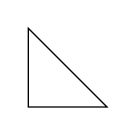
\begin{tikzpicture}
\draw (1,0) -- (0,0) -- (0,1) -- cycle;
\end{tikzpicture}

Jämför detta med syntaxen \verb+\draw (1,0) -- (0,0)  (0,1) -- (1,0);+

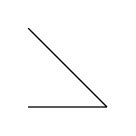
\begin{tikzpicture}
\draw (1,0) -- (0,0) (0,1) -- (1,0);
\end{tikzpicture}

Sammankoppling av två noder med räta vinklar sker med \verb+|-+ och \verb+-|+. Vi kan utläsa dessa som  att \verb+|+ motsvarar vertikal och \verb+-+ horisontell förflyttning, läst från vänster till höger. \verb+|-+ blir således ``först vertikalt, sedan horisontellt''.

\verb+\draw (0,0) |- (1,1)+\\
\verb+\draw (2,1) -| (3,0)+

\begin{tikzpicture}
\draw (0,0) |- (1,1) (2,1) -| (3,0);
\end{tikzpicture}

Kurvade vägar kan skapas genom Bézier-kurvor\footnote{http://sv.wikipedia.org/wiki/Bézier-kurva} med en eller två ankarpunkter med operationen ``..controls() ..()''.

\bve
\begin{tikzpicture}
\draw (0,0) .. controls (1,1) .. (4,0)
      (5,0) .. controls (6,0) and (6,1) .. (5,2);
\end{tikzpicture}
\end{verbatim}

\begin{tikzpicture}
\draw (0,0) .. controls (1,1) .. (4,0)
      (5,0) .. controls (6,0) and (6,1) .. (5,2);
\end{tikzpicture}

Vi kan även använda operationen ``to'' (utan parametrar motsvarar det \-\-). Tillsammans med parametrarna ``out'' och ``in'' kan vi skapa en krökt väg. Exempelvis får \verb+[out=135,in=45]+ en väg att lämna första koordinaten med en vinkel om 135 grader och ger en ankomst vid andra koordinaten i en vinkel om 45 grader.

\bve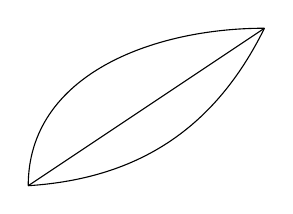
\begin{tikzpicture}
\draw (0,0) to (3,2);
\draw (0,0) to[out=90,in=180] (3,2);
\draw (0,0) to[bend right] (3,2);
\end{tikzpicture}\end{verbatim}

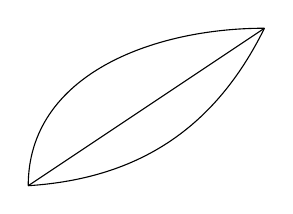
\begin{tikzpicture}
\draw (0,0) to (3,2);
\draw (0,0) to[out=90,in=180] (3,2);
\draw (0,0) to[bend right] (3,2);
\end{tikzpicture}

\subsection{Geometriska former}
Vidare finns även geometriska former, exempelvis ``rectangle'', ``circle'', ``ellipse'' och ``arc''. Dessa lämnas dock till läsaren att undersöka närmare, men vi ger ett exempel på hur ``rectangle'' kan användas:

\bve
\draw (0,0) rectangle (1,1);
\shade[top color=yellow, bottom color=black] (0,0) rectangle (2,-1);
\filldraw[fill=green!20!white, draw=green!40!black] (0,0) rectangle
(2,1);\end{verbatim}

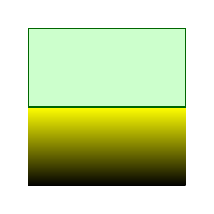
\begin{tikzpicture}
\draw (0,0) rectangle (1,1);
\shade[top color=yellow, bottom color=black] (0,0) rectangle (2,-1);
\filldraw[fill=green!20!white, draw=green!40!black] (0,0) rectangle
(2,1);
\end{tikzpicture}

\subsection{Grafer m.m.}
Utan att fördjupa oss alltför mycket ges här enstaka exempel på hur grafer kan skapas genom att använda olika operationer. Läsaren uppmuntras att antingen konsultera externa källor för närmare beskrivningar av dessa eller att kopiera dessa, ändra runt och se vad varje enskilt kommando gör. \TikZ är som sagt ett ofantligt stort bibliotek och det effektivaste sättet att lära sig det är ofta att möta varje problem när det uppstår.

\begin{verbatim}
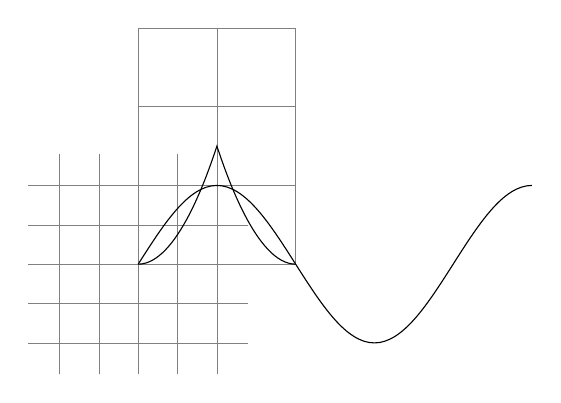
\begin{tikzpicture}
\draw[help lines] (0,0) grid (2,3);
\draw[step=0.5, gray, very thin] (-1.4,-1.4) grid (1.4,1.4);
\draw (0,0) parabola (1,1.5) parabola[bend at end] (2,0);
\draw (0,0) sin (1,1) cos (2,0) sin (3,-1) cos (4,0) sin (5,1);
\end{tikzpicture}
\end{verbatim}

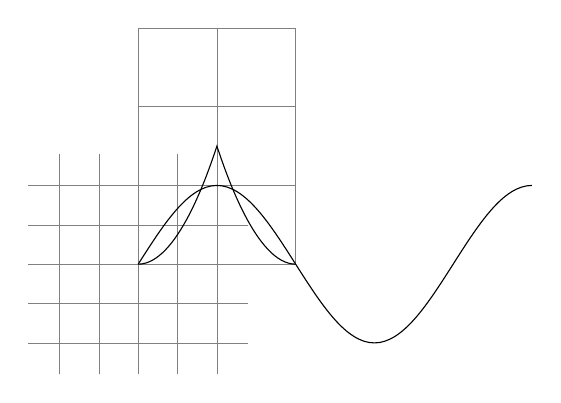
\begin{tikzpicture}
\draw[help lines] (0,0) grid (2,3);
\draw[step=0.5, gray, very thin] (-1.4,-1.4) grid (1.4,1.4);
\draw (0,0) parabola (1,1.5) parabola[bend at end] (2,0);
\draw (0,0) sin (1,1) cos (2,0) sin (3,-1) cos (4,0) sin (5,1);
\end{tikzpicture}

\begin{verbatim}
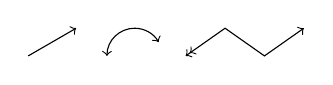
\begin{tikzpicture}
\draw [->] (0,0) -- (30:20pt);
\draw [<->] (1,0) arc (180:30:10pt);
\draw [<<->] (2,0) -- ++(0.5,10pt) -- ++(0.5,-10pt) -- ++(0.5,10pt);
\end{tikzpicture}
\end{verbatim}

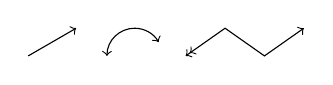
\begin{tikzpicture}
\draw [->] (0,0) -- (30:20pt);
\draw [<->] (1,0) arc (180:30:10pt);
\draw [<<->] (2,0) -- ++(0.5,10pt) -- ++(0.5,-10pt) -- ++(0.5,10pt);
\end{tikzpicture}

\begin{verbatim}
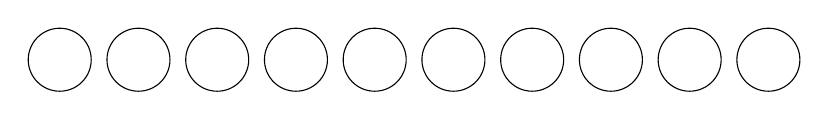
\begin{tikzpicture}
\foreach \x in {0,...,9}
\draw (\x,0) circle (0.4);
\end{tikzpicture}
\end{verbatim}

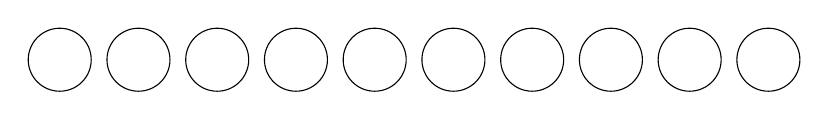
\begin{tikzpicture}
\foreach \x in {0,...,9}
\draw (\x,0) circle (0.4);
\end{tikzpicture}

\begin{verbatim}
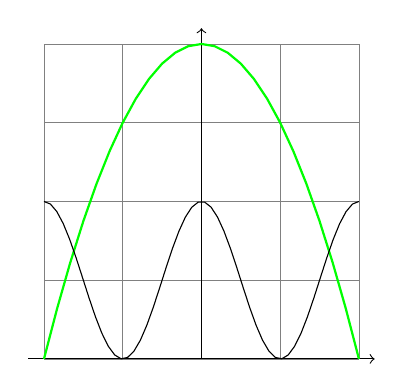
\begin{tikzpicture}
\draw [help lines] (-2,0) grid (2,4);
\draw[->] (-2.2,0) -- (2.2,0);
\draw[->] (0,0) -- (0,4.2);
\draw[green, thick, domain=-2:2] plot (\x, {4-\x*\x});
\draw[domain=-2:2, samples=50] plot (\x, {1+cos(pi*\x r});
\end{tikzpicture}
\end{verbatim}

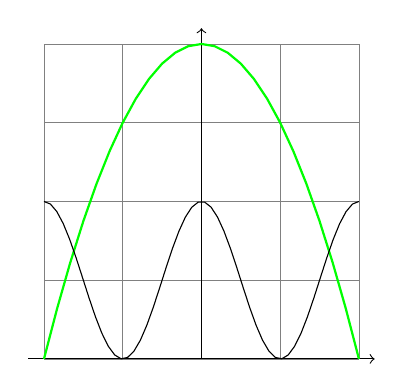
\begin{tikzpicture}
\draw [help lines] (-2,0) grid (2,4);
\draw[->] (-2.2,0) -- (2.2,0);
\draw[->] (0,0) -- (0,4.2);
\draw[green, thick, domain=-2:2] plot (\x, {4-\x*\x});
\draw[domain=-2:2, samples=50] plot (\x, {1+cos(pi*\x r});
\end{tikzpicture}

\begin{verbatim}
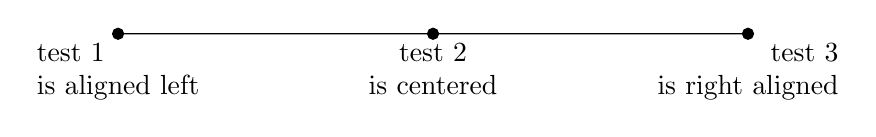
\begin{tikzpicture}
\filldraw
(0,0) circle (2pt) node[align=left,
below] {test 1\\is aligned
left} --
(4,0) circle (2pt) node[align=center, below] {test 2\\is centered}
--
(8,0) circle (2pt) node[align=right, below] {test 3\\is right
aligned};
\end{tikzpicture}
\end{verbatim}

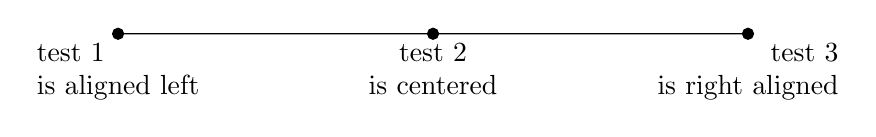
\begin{tikzpicture}
\filldraw
(0,0) circle (2pt) node[align=left,
below] {test 1\\is aligned
left} --
(4,0) circle (2pt) node[align=center, below] {test 2\\is centered}
--
(8,0) circle (2pt) node[align=right, below] {test 3\\is right
aligned};
\end{tikzpicture}


\chapter{Matematiktypsättning}\label{sec:math}
Matematisk typsättning är något WYSIWYG-editorer historiskt sett varit, och i mångt och mycket är än idag, dåliga på. \LaTeX{} gör det hela relativt enkelt, och inte minst konsekvent, och är måhända dess största styrka. Även utan vidare bibliotek har \LaTeX{} det mesta vi behöver för enklare matematiska formler, och med biblioteket \texttt{mathtools} får vi allt vi sannolikt behöver och lite till. \texttt{mathtools} inkluderar även biblioteket \texttt{amsmath} och således behöver inte båda inkluderas.

Då det här dokumentet inte avser att vara en komplett guide till \LaTeX{} kommer dock inte närmelsevis alla funktioner att behandlas. För detta hänvisas till referenslitteraturen.

Det första vi behöver veta för detta är att \LaTeX{} på förhand behöver veta att det som komma skall är matematiska element. Det beror på att \LaTeX{} hanterar matematisk notation annorlunda än vanlig text. För detta har vi två olika miljöer, beroende på hur de visas:
\itb
  \item \emph{text} - textformler visas i inuti texten,  $3x+2y=7z$ är ett exempel på detta.
  \item \emph{displayed} - formlerna är åtskilda från huvudtexten.
\ite
Till skillnad från de flesta miljöer finns ett par kortkommandon för att deklarera dessa \emph{``math modes''}:

\begin{tabular}{|l|l|l|p{9.5cm}|}
  \hline
  Typ & \emph{text} & \emph{displayed} & \emph{displayed} med automatisk numrering\\\hline
  Miljö & \texttt{math} & \texttt{displaymath} & \texttt{equation} \\\hline
  Kräver & & amsmath & amsmath\\\hline
  \LaTeX{}-syntax & \verb+\(...\)+ & \verb+\[...\]+ & \\\hline
  \TeX{}-syntax & \$\ldots\$ & \$\$\ldots\$\$ &\\\hline
\end{tabular}

\TeX-syntaxen bör i allmänhet undvikas, men fungerar för det mesta. AMS-LaTeX-makron kan, i synnerhet i kombination med \$\$\ldots\$\$ ställa till det och ge felmeddelanden som är svåra, om inte omöjliga, att tolka.

Math mode skiljer sig från ``vanligt'' läge på flera punkter:
\itb
\item Vita tecken (inklusive radbrytningar) ignoreras och härleds istället ur det matematiska uttrycket. De kan dock tvingas in med specifika kommandon.
\item Tomma rader är inte tillåtna. Endast ett stycke per formel.
\item Varje bokstav tolkas som namnet på en variabel och typsätts enligt detta. Detta kan överskuggas genom \verb+\mathrm{}+.
\ite

\section{Insättning av ``displayed'' i textblock}
Vissa kommandon, såsom \tb lim eller \tb sum, är exklusiva för math mode. Men inte nog med det, de kan även visas på ett oönskat vis. Det kan vara av intresse att använda \verb+\displaystyle+ för att få dessa att visas korrekt i löpande text. Exempelvis ger \verb+$\sum$+ ett $\sum$ medan \verb+$\displaystyle \sum$+ ger ett $\displaystyle \sum$ likt det i ekvationer. Detta kräver dock AMSMATH.

\section{Symboler}
Att lära sig vad matematiska symboler betyder är inte alltid så lätt, och att minnas hur man producerar dem i \LaTeX{} är nästan lika svårt. Det finns dock gott om listor online för just detta och vissa \LaTeX-editorer har även lättöverskådliga grafiska gränssnitt där dessa kan infogas med ett enkelt musklick, så någon lista på dessa kommer inte att omfattas av detta dokument. Det finns dock de flesta tänkbara operatorer, pilar och så vidare man kan behöva, exempelvis:

\verb+\forall x \in X, \quad \exists y \leq \epsilon+

$\forall x \in X, \quad \exists y \leq \epsilon$

\section{Grekiska bokstäver}
Grekiska bokstäver används ofta inom exempelvis matematiken och fysiken, och de är väldigt enkla att producera i math mode: ett \tb följt av bokstavens (engelska) namn. För gemener används inledande gemen, för versaler inledande versal. De som ser identiska ut med latinska bokstäver (ex. stort Alpha, Beta etc.) finns inte definierade i \LaTeX{} utan skrivs ut med dess latinska motsvarighet. Lilla epsilon, theta, phi, pi, rho och sigma, finns i två versioner. De alternativa \emph{var}ianterna skrivs då med ``var'' efter namnet.

\verb+\alpha, \beta, \gamma, \Gamma, \pi, \Pi, \phi, \varphi, \Phi+

$\alpha, \beta, \gamma, \Gamma, \pi, \Pi, \phi, \varphi, \Phi$

\section{Operatorer}
Operatorer skrivna som ord (ex. trigonometriska funktioner (sin, cos, tan) och logaritmer och exponentialfunktioner (log, exp)) har oftast fördefinierade kommandon:

\verb+\cos (2\theta) = \cos^2 \theta - \sin^2 \theta+
$\cos (2\theta) = \cos^2 \theta - \sin^2 \theta$

\section{Exponenter och index}\label{sec:mathexp}
Exponenter och index i math mode är lite bekvämare än i normal text\footnote{Det kommer dock att typsättas enligt math mode, så använd upphöjt och nedsänkt läge enligt avsnitt \ref{sec:textexp}, sid \pageref{sec:textexp} för normal text.}. För exponenter använder vi \verb+^{}+ och \verb+_{}+ och placerar det som ska upphöjas eller nedsänkas inom måsvingarna. Om endast ett tecken ska justeras kan måsvingarna utelämnas.

\section{Bråk och binomial}
Bråk skapas genom \verb+\frac{täljare}{nämnare}+. Binomial skrivs på samma sätt med \verb+\binom{}{}+:

\verb+\frac{n!}{k!(n-k)!} = \binom{n}{k}+

$\frac{n!}{k!(n-k)!} = \binom{n}{k}$

Bråk kan även nästlas i andra bråk:

\verb?\frac{ \frac{1}{x}+\frac{1}{y} } {y-z}?

$\frac{\frac{1}{x}+\frac{1}{y}}{y-z}$

Snedställda bråk ($\sfrac{1}{2}$) kan skrivas med \verb+\sfrac+ (\verb+\usepackage{xfrac}+)

Kedjebråk bör skrivas med \verb+\cfrac+:

\begin{verbatim}
  x = a_0 + \cfrac{1}{a_1
    + \cfrac{1}{a_2
      + \cfrac{1}{a_3 + \cfrac{1}{a_4} } } }
\end{verbatim}

$  x = a_0 + \cfrac{1}{a_1
    + \cfrac{1}{a_2
      + \cfrac{1}{a_3 + \cfrac{1}{a_4} } } }$

\section{Rotuttryck}
Rotuttryck skrivs med \verb+\sqrt[]{}+:

\verb+\sqrt[a]{b}+ {\Large\quad$\sqrt[a]{b}$}

\section{Summor och integraler}
Kommandona \verb+\sum+ och \verb+\int+ sätter in summatecken och integraltecken med gränser specifierade med (\textasciicircum) och (\_).

\verb+\sum_{i=1}^{10} t_i+

$\sum_{i=1}^{10} t_i$
\\\\
I \emph{text}-mode \verb+\[...\]+ kommer \LaTeX{} att typsätta gränserna enligt ovan för att spara radhöjt. Om vi i stället använder \emph{displayed} kommer den standardvarianten att väljas:

$\displaystyle\sum_{i=1}^{10} t_i$

Vill vi tvinga fram detta i \emph{text} utan att använda \verb+\displaystyle+ (om vi vill ha kvar det mindre summatecknet) kan vi göra detta med \verb+\underset{}{}+ och \verb+\overset{}{}+:

\verb+\underset{i=1}{\overset{10}{\sum}} t_i+

$\underset{i=1}{\overset{10}{\sum}} t_i$

Sistnämnda variant fungerar även för \tb int, men det finns en enklare lösning -- \verb+\int\limits+:

\verb+\int\limits_a^b+

$\displaystyle \int\limits_a^b$

\section{Automatisk storlek}\label{sec:lrm}
Ofta skiljer sig matematiska element i storlek varvid exempelvis parenteser bör justeras för att passa uttrycket. Det kan göras med kommandona \verb+\left, \right, \middle+. Om ett avgränsande tecken (delimiter) endast används på en sida av ett uttryck används en osynlig delimiter (.) på andra sidan. Några exempel:

\verb+\left(\frac{x^2}{y^3}\right)+

$$\left(\frac{x^2}{y^3}\right)$$

\verb+P\left(A=2\middle|\frac{A^2}{B}>4\right)+

$$P\left(A=2\middle|\frac{A^2}{B}>4\right)$$

\verb+\left\{\frac{x^2}{y^3}\right\}+

$$\left\{\frac{x^2}{y^3}\right\}$$

\verb+\left.\frac{x^3}{3}\right_0^1+

$$\left.\frac{x^3}{3}\right|_0^1$$

\section{Matriser}
Matriser kan skapas genom miljön \verb+matrix+\footnote{kräver amsmath}. I likhet med exempelvis \verb+tabular+ anger vi elementen separerade radvis med \tb\tb{} och kolumnerna separerade med ampersand (\&). Kolumnjustering (lcr) kan anges som parameter om vi använder \verb+matrix*+\footnote{kräver mathtools} (standard = c):

\bve
\begin{matrix*}[r]
  a & b & -c \\
  d & -e & f \\
  -g & h & i
\end{matrix*}
\end{verbatim}

$\begin{matrix*}[r]
  a & b & -c \\
  d & -e & f \\
  -g & h & i
\end{matrix*}$

Matriser har oftast någon form av delimiter. Vi kan använda \verb+\left+ och \verb+right+ för detta, men det finns även fördefinierade miljöer som automatiskt inkluderar dessa. Samtliga kommer i mathtools med *-motsvarigheter: pmatrix (), bmatrix \lbrack{} \rbrack, Bmatrix \{\}, vmatrix \verb+|+ och Vmatrix \verb+||+.

För matriser av godtycklig storlek kan \verb+\cdots, \vdots, \ddots+ användas.

\bve
A_{m,n} =
\begin{pmatrix}
  a_{1,1} & a_{1,2} & \cdots & a_{1,n} \\
  a_{2,1} & a_{2,2} & \cdots & a_{2,n} \\
  \vdots & \vdots & \ddots & \vdots \\
  a_{m,1} & a_{m,2} & \cdots & a_{m,n}
\end{pmatrix}
\end{verbatim}

$A_{m,n} =
\begin{pmatrix}
  a_{1,1} & a_{1,2} & \cdots & a_{1,n} \\
  a_{2,1} & a_{2,2} & \cdots & a_{2,n} \\
  \vdots & \vdots & \ddots & \vdots \\
  a_{m,1} & a_{m,2} & \cdots & a_{m,n}
\end{pmatrix}$

Vid exempelvis bråktal lämnar inte alltid matrix-klassen tillräckligt med utrymme mellan raderna. Detta kan hjälpas med en extra parameter efter \tb\tb: \verb+\\[0.3mm]+

\section{Övrigt}
Som säkert märkts är matematisk typsättning omständligt, och mer finjustering än vad som tagits upp här står att finna, men det är inte särskilt svårt. Det här dokumentet avser, återigen, inte att vara heltäckande på något sätt, och framför allt inte gällande just detta avsnitt. Avsikten är att snabbt komma igång, belysa potentialen och att ge ett hum om vad som kan åstadkommas med hjälp av \LaTeX.


\chapter{Kemi, teknik etc.}\label{sec:kemi}
\LaTeX{} är inte bara en bra grund att bygga dokument med matematik i. Genom åren har \LaTeX{}:s utomordentliga grund för akademiska texter kommit att inspirera mängder av expansionsbibliotek - vissa är bättre, andra bjuder fortfarande på en hel del buggar - och idag kan man i stort sett hitta stöd för typsättning och layout för vad man än kan tänka sig. Det här avsnittet ämnar inte att behandla detaljer kring några specifika bibliotek. Däremot kommer några få uppslag på vad som finns i avseende, i likhet med kapitel \ref{sec:math}, att belysa möjligheter för att bredda läsarens inspiration.

Om just ditt ämnesområde har ett behov som inte tas upp här eller på annat ställe i detta dokument, tveka inte att söka runt på nätet.

\section{Kemi}
Kemi är ofta en mardröm att typsätta för den som inte är bekant med \LaTeX{}. Det finns två stora bibliotek för att underlätta det hela: \verb?ochem?\footnote{\url{http://www.2k-software.de/ingo/ochem.html}} och \verb?chemfig?. Det här dokumentets sammanställare kan dock inte svara för ochems kapacitet. Chemfig använder \TikZ{} för att producera grafiska representationer på ett lättscriptat vis. För exempel och handledning hänvisas till bibliotekets dokumentation\footnote{\url{http://mirror.ctan.org/macros/latex/contrib/chemfig/chemfig_doc_en.pdf}}.

\section{Elektronik och digitalteknik}
Det finns gott om god extern programvara för att skapa exempelvis kopplingsscheman och för mer komplexa projekt kan dessa oftast vara att föredra i kombination med import av exporterade bilder till \LaTeX{}-dokumentet. För mindre projekt kan dock exempelvis \verb?circuitikz?\footnote{http://http://texdoc.net/texmf-dist/doc/latex/circuitikz/circuitikzmanual.pdf} vara lämpligt. Som namnet antyder bygger det på \TikZ{} och erbjuder ett stort utbud på symboler.

\section{Presentationer och examinationer}
Vant dig vid att fixa allt mellan himmel och jord i \LaTeX{} och vill skapa även dina overhead-slides på WYSIWYM-manér? Ta en titt på \verb?beamer?\footnote{\url{http://www.ctan.org/tex-archive/macros/latex/contrib/beamer/}}\footnote{\url{https://tug.org/TUGboat/tb26-1/mertz.pdf}} och lär dig hur du äntligen kan göra dig kvitt Powerpoint utan att behöva ge upp handout-sammanställningar eller förlita dig på statiska dokument.

Med dokumentklassen \verb?exam? får man tidseffektivt inte bara ett enhetligt utseende som gör eleverna bekanta med en typsättning många av dem kommer att stöta på om och om igen under sina tentamenstillfällen på högskolenivå, man slipper även hålla ordning på två dokument för varje examination (dels examinationen, dels svarsmallar/lösningsexempel). Möjlighet att poängsätta och numrera varje uppgift ingår givetvis, likaså att sömlöst infoga allt annat \LaTeX{} bjuder på.


\chapter{Referenshantering}\label{sec:referenser}
Varje akademiker värd namnet känner till vikten av referenser. Varje akademiker värd namnet och som inte använt \LaTeX{} känner till \emph{vikten} av referenshantering.

\LaTeX{} kan givetvis med enkla grepp som vi redan lärt oss hantera enklare referenshantering med fotnoter, men det kräver fortfarande att man håller reda på sina källor själv. Det finns idag mången programvara som kan underlätta det hela, såväl online som offline, men få (som inte bygger på BibTeX) som når lika långt och sömlöst som BibTeX går ihop med \LaTeX.

BibTeX håller alla de verk man sparar i en databas. Den databasen kan i sin tur sedan länkas till i godtyckligt \LaTeX-dokument och citat göras till valfri referens i databasen. Givetvis kan man även spara verken i multipla databaser om så önskas även om det troligen är mest aktuellt för den som redan sysslar med forskning och således sannolikt redan är bekant med BibTeX.

Mitt emellan dessa två finner vi dessutom \LaTeX:s inbyggda system, \verb?thebibliography?. Det är måhända det mest aktuella för allt under examensarbetesnivå då mängden litteratur fortfarande är hanterbar manuellt och då det inte direkt finns någon vinst tidsmässigt med BibTeX.

\section{Användning av thebibliography}
\subsection{Litteraturförteckning}
\LaTeX skeppas med en miljö kallad \verb?thebibliography? som används där man vill ha sina källor (vanligtvis mot slutet av dokumentet). Vi hoppar direkt på ett exempel:

\begin{verbatim}
\begin{thebibliography}{9}

\bibitem{lamport94}
Leslie Lamport,
\emph{\LaTeX: A Document Preparation System}.
Addison Wesley, Massachusetts,
2nd Edition,
1994.

\end{thebibliography}
\end{verbatim}

Vad händer då här? Först och främst skapar vi miljön, i det här fallet med parametern \{9\}. Det innebär att vi begränsar litteraturförteckningen till 9 element, men det är inte siffran i sig som avgör det. Parametern ``3'' hade gett samma resultat; det är alltså \emph{antalet siffror} som avgör antalet källor. ``34'' möjliggör exempelvis 99 källor.

I och med att vi skapar denna miljö skapar vi även ett nytt kapitel som kommer att\footnote{under förutsättning att vi satt svenska som språk -- \tb usepackage\lbrack swedish\rbrack\{babel\}} få titeln ``Litteraturförteckning''.

Därefter kommer själva verket vilket inleds med en citeringsnyckel (\verb?\bibitem{cite_key}?) som skall vara en unik identifierare för just det verket. Citeringsnyckeln får innehålla A-Z, a-z, 0-9 och vissa skiljetecken (ej kommatecken). Normen är att ange författarensnamn och årtalet, samt en extra bokstavsnumrering om författaren varit flitig ett visst år. Men det är givetvis upp till var och en att avgöra hur man vill sköta det, även om en standard kan vara på sin plats vid kollaborativt skrivande.

Därefter kommer det som ska skrivas ut i litteraturförteckningen. Du måste skriva det som du vill ha det presenterat. Vi har här gett elementen egna rader för läsbarhetens skull, men i sedvanlig ordning ignoreras dessa radbrytningar av \LaTeX.

\subsection{Citat och referenser}
Nog för att vi nu har en fin litteraturförteckning, men den kommer inte göra mycket nytta om den inte hänvisas till. Tyvärr kommer den akademiska världen med flera olika standarder gällande hur man anger källor, och för att krångla till det är alla inte alltid konsekventa med namnen på dessa. De termer som används i detta dokument är dock följande:
\itb
  \item Oxfordsystemet: fotnotsreferenser
  \item Vancouversystemet: siffra inom hakparentes med numrerad litteraturförteckning
  \item Harvardsystemet: författare och år inom bågparenteser
\ite

Utan handpåläggning kommer vancouversystemet att användas, men nedan nämns även kort hur harvardsystemet kan implementeras. Låt oss dock börja från början.

För att citera en källa använder vi oss av \texttt{\tb cite\{\emph{cite\_key}\}}, där \emph{cite\_key} är det ``bibitem'' vi citerar. När \LaTeX{} processar dokumentet kommer, i likhet med andra former av interna referenser, att korsreferera mot vår litteraturlista och hålla ordning på numreringen. Tänk dock på att det kan behöva kompileras en extra gång, av samma anledning som vår innehållsförteckning.

Vill vi sedan ange ett sidonummer kan vi lägga till det som parameter (\verb?\cite[sid.~215]{cite_key}?) och vill vi ange flera källor använder vi endast ett \verb?\cite{}? men med kommateckensseparerade (utan mellanslag) argument.

\subsection{Natbib}
Vancouversystemet är vanligt på de tekniska fakulteterna, men det finns hopp även för de som är hänvisade till harvardsystemet. Detta möjliggörs genom \verb?natbib?. Undertecknad har inte lyckats få det att fungera ihop med ``thebibliography'', men tillsammans med BibTeX kan vi utan problem överskugga det inbakade vancouversystemet med en uppsättning alternativa kommandon\footnote{\url{http://en.wikibooks.org/wiki/LaTeX/Bibliography_Management\#Natbib}} för att få harvardsystemets referensmodell. 

\subsection{BibTeX}
BibTeX använder en stiloberoende textbaserad databas för att spara referenser. Filformatet slutar vanligen på .bib och exempel på mjukvaror har ges i avsnitt \ref{sec:refsoft} (sid. \pageref{sec:refsoft}). BibTeX och dess implementering i \LaTeX ställer en del krav på noggrannhet och vid en första anblick kan det verka som att det är väldigt mycket att hålla koll på. Det är dock relativt lätt att hitta exempelmallar på själva implementeringen, och därefter är det bara att se till att de obligatoriska uppgifterna för verk refererade i aktuell typ av dokument är inskrivna i databasen. För en mer detaljerad introduktion till BibTeX hänvisas till referenslitteratur\footnote{\url{http://en.wikibooks.org/wiki/LaTeX/Bibliography_Management\#BibTeX}}


\appendix
\chapter{Appendix}\label{sec:appendix}
        \section{Kommandon}\label{sec:kommandon}
        Det här är en avkortad lista över \LaTeX{}-kommandon med en kort sammanfattning över dess funktionalitet. Hakparenteser ``\lbrack{}\rbrack{}'' är valfria parametrar, måsvingar ``\{\}'' är obligatoriska argument. Vissa kommandon har inte berörts tidigare och det lämnas åt läsaren att själv antingen pröva sig fram till dess funktionalitet eller söka sig till fördjupad information om dessa. Detta dokument avser, som tidigare nämnts, inte att vara en komplett sammanfattning av \LaTeX{}.

\subsection{\#}
\cc{@}{avslutar mening efter punkt}
\cc{\tb\lbrack\*\rbrack\lbrack{}extra avstånd\rbrack{}}{nyrad}
\cc{,}{kort mellanslag}
\cc{;}{långt mellanslag, math mode}
\cc{!}{kort negativt mellanslag, mathmode}
\cc{-}{avstavning}
\cc{'}{accent på nästkommande tecken}
\cc{|}{dubbla vertikala linjer, mathmode}
\cc{(}{starta mathmode}
\cc{)}{avsluta mathmode}
\cc{\lbrack}{starta displaymath}
\cc{\rbrack}{avsluta displaymath}

\subsection{A}
\cc{addcontentsline\{file\}\{sec\_unit\}\{entry\}}{lägger till en post till specifierad lista eller tabell}
\cc{addtocontents\{file\}\{text\}}{lägger till text eller formatteringskommandon direkt till den fil som skapar specifierad lista eller tabell}
\cc{addtocounter\{counter\}\{value\}}{inkrementerar specifierad räknare}
\cc{addvspace}{lägger till vertikalt utrymme av specifierad höjd}
\cc{alph}{skriver ut värdet av en räknare med bokstäver}
\cc{appendix}{ändrar sektionsinställningar till att räknas som appendix}
\cc{arabic}{skriver ut värdet av en räknare med siffror}
\cc{author\{\}}{deklarerar dokumentets författare}

\subsection{B}
\cc{backslash}{skriver ut ett \tb i mathmode}
\cc{bf}{fetstil}
\cc{bibitem}{skapar etikett för litteraturförteckning}
\cc{boldmath}{fetstil i mathmode}

\subsection{C}
\cc{cal}{kalligrafisk stil i mathmode}
\cc{caption}{skapar annotation för figurer och tabeller}
\cc{cdots}{centrerade punkter ($\cdots$), mathmode}
\cc{centering}{centrering av \LaTeX-miljöer}
\cc{chapter}{påbörjar nytt kapitel}
\cc{cite}{använder bibitem för att hänvisa till litteraturförteckningen}
\cc{cleardoublepage}{skriver ut cachens eventuella floats etc. och avslutar aktuell sida}
\cc{clearpage}{som cleardoublepage men för enkelsida}
\cc{cline}{begränsad horisontell linje, se hline och kap. \ref{sec:grafik}}
\cc{color}{färgsätter text}
\cc{copyright}{skapar \copyright}

\subsection{D}
\cc{date}{definierar datum}
\cc{ddots}{$\ddots$ i mathmode}
\cc{documentclass\lbrack\rbrack\{style\}}{används för att påbörja ett \LaTeX-dokument}
\cc{dotfill}{fyller med punkter, som i denna lista}

\subsection{E}
\cc{em}{växelkommando för kursiv stil}
\cc{emph\{\}}{kursiverar/inverterar kursiverad stil}

\subsection{F}
\cc{footnote\{\}}{skapar fotnot}
\cc{frac\{\}\{\}}{skapar bråktal}
\cc{frenchspacing}{motverka längre mellanrum efter punkt}

\subsection{H}
\cc{hfill}{som dotfill utan punkter}
\cc{hline}{horisontell linje i tabular-miljön}
\cc{hrulefill}{som dotfill men med heldragen linje}
\cc{hspace}{skapa horisontellt mellanrum}
\cc{huge}{en större teckensnittsstorlek än \tb{}LARGE}
\cc{Huge}{en ännu större teckensnittsstorlek}

\subsection{I}
\cc{include}{skiljer sig från \tb{}input i det att det inkluderar outputen i stället för kommandona från andra filer}
\cc{includegraphics}{infogar en bild, kräver graphicx}
\cc{indent}{infoga indentering}
\cc{input}{läs in och inkludera en annan \LaTeX-fil}
\cc{item}{skapar en punkt i en lista}

\subsection{L}
\cc{label}{skapar en etikett som sedan kan refereras till via \tb{}ref och \tb{}pageref}
\cc{large}{en stor teckensnittsstorlek}
\cc{Large}{en större teckensnittsstorlek}
\cc{LARGE}{en ännu större teckensnittsstorlek}
\cc{LaTeX}{skriver ut \LaTeX{}}
\cc{ldots}{skriver ut ``\ldots{}'' med adekvat typsättning}
\cc{left}{se sid. \pageref{sec:lrm}}
\cc{linebreak}{föreslår radbrytning för \LaTeX}
\cc{listoffigures}{infogar figurlista, jmf. med innehållsförteckning}
\cc{listoftables}{infogar tabellista}

\subsection{M}
\cc{maketitle}{typsätter och infogar förstasida}

\subsection{N}
\cc{newcommand\lbrack\rbrack\{\}}{definiera nytt kommando}
\cc{newcounter}{definiera en ny räknare}
\cc{newenvironment}{definiera en ny miljö}
\cc{newline}{infoga nyrad}
\cc{newpage}{infoga sidbrytning}
\cc{noindent}{motverka indentering av denna rad}
\cc{nonfrenchspacing}{stänger av frenchspacing}
\cc{normalsize}{återgår till normal teckenstorlek}
\cc{nopagebreak}{föreslår för \LaTeX{} att inte sidbryta här}

\subsection{O}
\cc{overbrace}{infogar $\overbrace{\mathrm{overbrace}}$ i mathmode}

\subsection{P}
\cc{pagebreak}{föreslår sidbrytning}
\cc{pagenumbering}{definierar typ av sidnumrering (arabic, roman, Roman, alph, Alph, gobble)}
\cc{pageref}{returnerar sidnumret där motsvarande ``\tb{}label'' finns}
\cc{pagestyle}{definierar sidlayout}
\cc{par}{startar nytt stycke}
\cc{paragraph}{startar nytt namnsatt stycke}
\cc{parindent}{indenterar nya stycken}
\cc{parskip}{nyrad för nya stycken}
\cc{part}{ny del, se \ref{sec:sections} sid. \pageref{sec:sections}}

\subsection{R}
\cc{ref}{returnerar returvärde av ``\tb{}label''}
\cc{renewcommand}{omdefinierar ett kommando}
\cc{right}{se sid. \pageref{sec:lrm}}
\cc{rm}{växel för standardteckensnitt}
\cc{rule}{infogar linje av specifierad längd och höjd}

\subsection{S}
\cc{sc}{växel för \sc{}kapitäler\sc{}}
\cc{section\{\}}{ny section}
\cc{setcounter}{sätt en counter till specifierat värde}
\cc{sf}{växel för \sf{}sans serif\sf{}}
\cc{sl}{växel för \sl{}slanted\sl{}}
\cc{small}{liten teckenstorlek}
\cc{sqrt}{infogar rottecken}
\cc{stepcounter}{inkrementerar en räknare}
\cc{subparagraph}{ny subparagraph}
\cc{subsection}{ny subsection}
\cc{subsubsection}{ny subsubsection}

\subsection{T}
\cc{tableofcontents}{infogar innehållsförteckning}
\cc{TeX}{infogar \TeX-logo}
\cc{textbf}{fetstilt text}
\cc{textcolor\{\}\{\}}{färgad text}
\cc{textit}{kursiv text}
\cc{textnormal}{normal text}
\cc{textrm}{standardtext}
\cc{textsc}{text i kapitäler}
\cc{textsl}{text i \textsl{slanted}}
\cc{texttt}{text med \texttt{fast teckenbredd}}
\cc{thispagestyle}{definierar sidlayout för aktuell sida}
\cc{tiny}{mindre teckenstorlek än small}
\cc{title}{definierar titelnamn}
\cc{today}{infogar dagens datum}
\cc{tt}{växel för fast teckenbredd}

\subsection{U}
\cc{underbrace\{\}}{infogar $\underbrace{\mathrm{underbrace}}$ i mathmode}
\cc{underline\{\}}{infogar $\underline{\mathrm{underline}}$ i mathmode}

\subsection{V}
\cc{vdots}{infogar $\vdots$ i mathmode}
\cc{verb}{skapar verbatim inline}
\cc{vfill}{infogar vertikalt mellanrum, jmf. hfill}
\cc{vline}{infogar vertikal linje}



\section{Paket}\label{sec:paket}

Författaren har haft för avsikt att på de ställen där exempelkommandon förekommit ange nödvändiga paket. Dock kan missar ha smugit sig in. För att täcka upp för dessa ges därför här en komplett lista på de paket som behövs för att kompilera samtlig kod angiven i detta dokument fram till, men ej inkluderande, \ref{sec:appendix} Appendix. Skulle någon miss hittas, anmäl gärna detta till tidigare angiven mailadress.

\texttt{titlesec, tikz, textcomp, fixltx2e, color, fullpage, graphicx, afterpage, float, parskip, mathtools, xfrac}


